\subsection{Voor een aanbevelingsaanvraag}
\label{voor_aanvraag}

\begin{center}
\centering
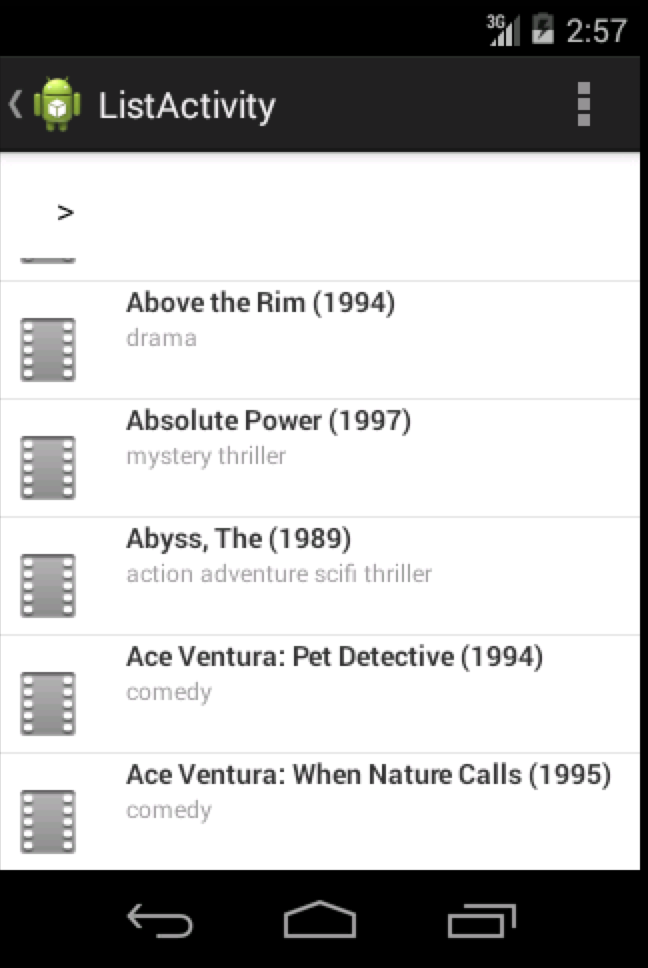
\includegraphics[scale=0.5]{fig/all_items} 
\captionof{figure}{De gebruiker krijgt de lijst met films te zien uit de MovieLensdatabase} 
\label{all_items}
 
\end{center}

\begin{center}
\centering
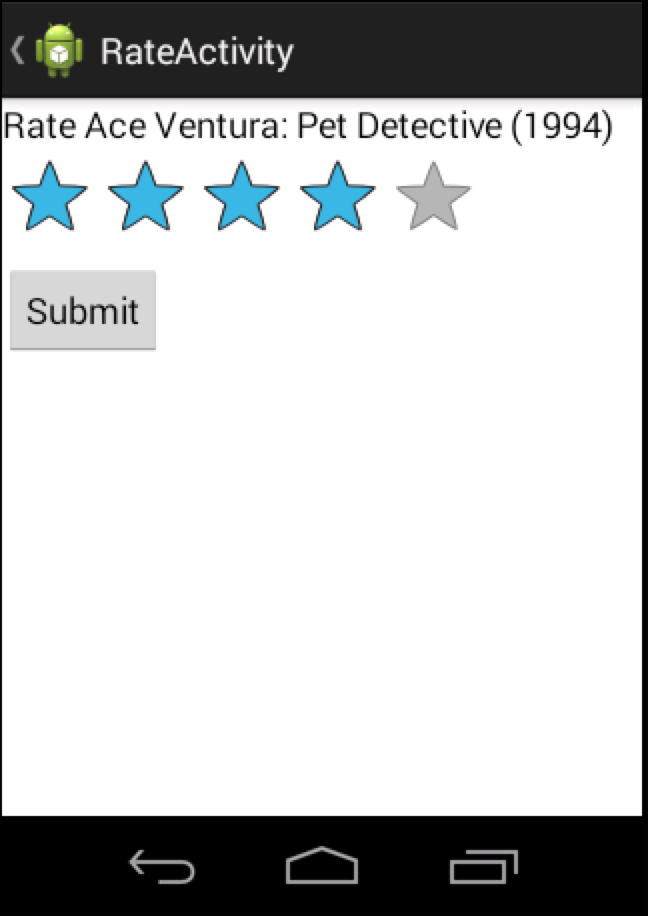
\includegraphics[scale=0.5]{fig/rate_item}
\captionof{figure}{De gebruiker beoordeelt een film.} 

    \label{rate_item} 
 
\end{center}
Voor een aanbevelingsaanvraag zal de gebruiker verschillende items beoordelen. De ratings worden lokaal bijgehouden in de Androidapplicatie in een SQLiteDatabase. Ze worden daarna voor het sturen van het profiel ge\"encrypteerd met de publieke sleutel van het Pailliersysteem van de controleserver en naar de recommenderserver gestuurd. \\Om de gelijkenis te berekenen tussen twee gebruikers wordt er dezelfde methode gebruikt als in \ref{cryptoprotocollen} en wordt de Pearson-co\"efficient dus opgesplitst \eqref{similarity}.\\ 
Per gebruiker moeten dus de \emph{preferences} of C-waarden $C_{X,i}$ bepaald worden. De preferences worden bepaald op basis van de ratings van een bepaalde deelverzameling van de items. Deze deelverzameling wordt het best bepaald door items te nemen die door het gros van de gebruikers beoordeeld zijn. Om deze lijst dynamisch te bepalen zou de recommenderserver moeten weten hoeveel gebruikers een bepaald item ge\"evalueerd hebben. Dat kan niet dynamisch bepaald worden gezien het volledig privacyvriendelijk karakter van dit systeem. Hierdoor mag de server niet weten welke gebruiker welk item beoordeeld heeft, zelfs al weet de server de waarde van de beoordeling niet.
Dit zou contact kunnen verraden tussen een user en een item, bijvoorbeeld dat een persoon naar een restaurant geweest is.
Het systeem zou met deze data zelfs een smakenprofiel van een gebruiker opzetten. Een oplossing voor dit probleem is de deelverzameling vast kiezen en eventueel bij het eerste gebruik aan de gebruiker vragen deze lijst te evalueren, zonder hem te verplichten een bepaald item te raten. Deze deelverzameling zou dan best opgesteld worden uit items waarover de mening van de gebruikers verdeeld is en niet diegene die de meeste users goed of slecht vinden. 

De  $\bar{v}_X$ en $\sqrt{\sum_{j=0}^{M-1} (v_{(X,j)} - \bar{v}_X)^2}$ waarden zijn voor elke C-waarde gelijk. Dit betekent dat je de C-waarde eventueel ook aan de kant van de server zou kunnen berekenen en voor de deling in het Pailliersysteem gebruik maken van een protocol als \cite{VeugenEID}. Dit lijkt niet zo effici\"ent en er werd besloten de berekening van de C-waarden te doen op de client en ge\"encrypteerd mee te sturen in het profiel.
\begin{figure}[htpb]   
    \label{Figuur::upload_profile}      
  \begin{center}    
 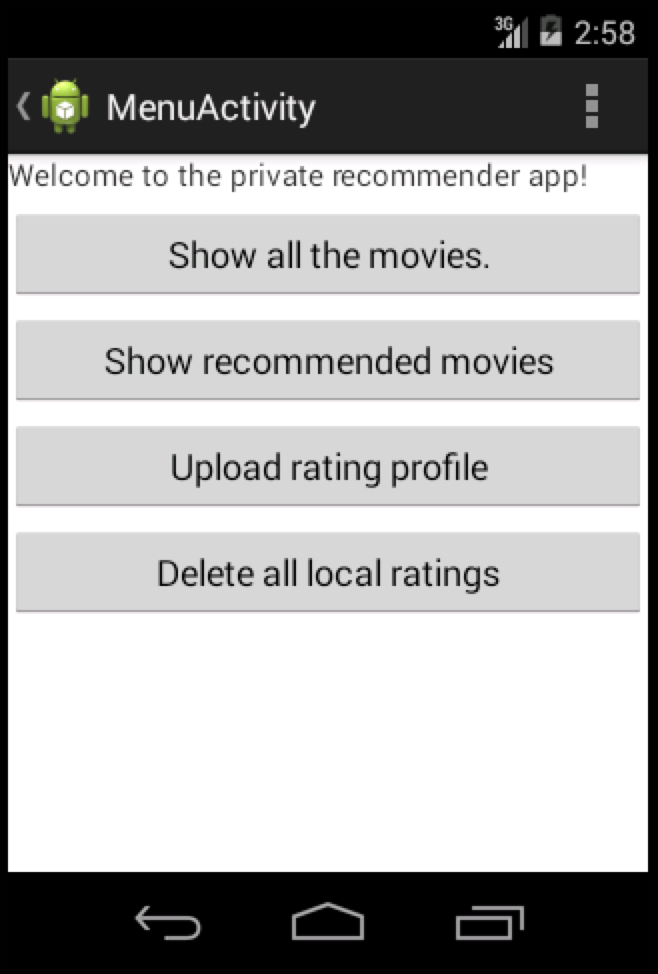
\includegraphics[scale=0.5]{fig/upload_profile}    
  \end{center}   
  \caption{Het menu van de testapplicatie. De gebruiker kan zijn profiel uploaden wanneer hij wil.}  
   \end{figure}
Naast de lijsten van de ratings en de preferences geven we ook nog een lijst ge\"encrypteerde bits mee die aangeven of een item wel (1) of niet (0) beoordeeld is door deze gebruiker. Dit lijkt redundante informatie maar dit kunnen we gebruiken als we moeten optellen hoeveel (ingevulde) ratings er werden opgeteld.  Dat komt omdat als we het profiel naar de server sturen ook "ratings" moeten doorsturen van items die de persoon nog niet beoordeeld heeft. Dit om te verbergen welke items de persoon ge\"evalueerd heeft. Dit is een uitbreiding op de theoretische paper \cite{ZErkinDyn} waar er enkel de beoordeelde waarden naar de server gestuurd worden. We sturen ook best de waarden van alle items mee, anders zitten er C-waarden in de databank op de server berekend op verouderde $\bar{v}_X$ en $\sqrt{\sum_{j=0}^{M-1} (v_{(X,j)} - \bar{v}_X)^2}$ waarden. Deze manier geeft ook de garantie op de hoogste privacy. Een andere optie is om als gebruiker een paar random items te kiezen en enkel voor deze items een nulwaarde te encrypteren. Indien al deze items van hetzelfde soort zijn, krijgt de server nog altijd persoonlijke data. Bijvoorbeeld als er in de MovieLens database, allemaal komedies worden gekozen, kan dat nog steeds de voorkeur verklappen van een persoon voor komedies. Daarom worden in dit geval de best items slim gekozen.

We geven ook de gebruiker de keuze wanneer hij zijn profiel uploadt en hij kan ook zijn lokale ratings leegmaken. Dit geeft hem meer controle over zijn profiel en laat hem toe om zijn profiel eerst leeg te maken en dan up te loaden. Zo heeft de aanbevelingsserver geen enkele ge\"encrypteerde beoordeling meer staan van deze gebruiker, tenzij hij natuurlijk backups nam. Het bespaart ook data-overdracht en processortijd als de upload niet bij elke rating gebeurt.

Nu moet er de keuze gemaakt worden wanneer de encryptie gebeurt. De encryptie gebeurt optimaal op het moment dat het profiel wordt gestuurd naar de aanbevelingsserver en niet alvorens de rating in de databank wordt geplaatst. Dit is aan de ene kant logisch aangezien ook de C-waarden dan het best berekend worden met de laatste waarden, maar zorgt er ook voor dat alle ge\"encrypteerde waarden telkens anders zijn zodat de server niet kan zien welke waarden veranderd zijn ten opzichte van een vorige rating dankzij de semantische veiligheid van het Paillier-cryptosysteem.